\begin{figure}[t]
  \hspace{0.05\textwidth}%
  \begin{subfigure}[b]{\textwidth}
    \tikzstyle{legend-point}=[circle, inner sep=2pt]
    \definecolor{GraphBlue}{HTML}{6c8abd}
    \definecolor{GraphGreen}{HTML}{73b584}
    
    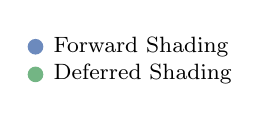
\begin{tikzpicture}
      %\node (forward) at (0,0) [fill={GraphBlue}] {};
      \node (legend:forward) at (0.1\textwidth,0) [legend-point, fill={GraphBlue}, label=right:{\footnotesize Forward Shading}] {};
      \node (legend:deferred) at (0.1\textwidth, -10pt) [legend-point, fill={GraphGreen}, label=right:{\footnotesize Deferred Shading}] {};
    \end{tikzpicture}
  \end{subfigure}\hfill\\
  \begin{adjustbox}{minipage=\textwidth, scale=0.55}
    \begin{subfigure}[b]{0.8\textwidth}
      \centering
      \def\svgwidth{\textwidth}
      \input{./img/raw/fds-frames/spaceship-indoor/frames_320_70.pdf_tex}
      \caption{Spaceship indoor: $70$ lichten, $320^2$ pixels.}
      \label{fig:fds-test-frames:indoor-low}
    \end{subfigure}
  \end{adjustbox}\hspace{-0.075\textwidth} %
  %
  \begin{adjustbox}{minipage=\textwidth, scale=0.55}
    \begin{subfigure}[b]{0.8\textwidth}
      \centering
      \def\svgwidth{\textwidth}
      \input{./img/raw/fds-frames/spaceship-indoor/frames_2560_1260.pdf_tex}
      \caption{Spaceship indoor: $1260$ lichten, $2560^2$ pixels.}
      \label{fig:fds-test-frames:indoor-high}
    \end{subfigure}
  \end{adjustbox} \\
  %
  \begin{adjustbox}{minipage=\textwidth, scale=0.55}
    \begin{subfigure}[b]{0.8\textwidth}
      \centering
      \def\svgwidth{\textwidth}
      \input{./img/raw/fds-frames/pipers-alley/frames_320_58.pdf_tex}
      \caption{Pipers Alley: $58$ lichten, $320^2$ pixels.}
      \label{fig:fds-test-frames:alley-low}
    \end{subfigure}
  \end{adjustbox}\hspace{-0.075\textwidth} %
  %
  \begin{adjustbox}{minipage=\textwidth, scale=0.55}
    \begin{subfigure}[b]{0.8\textwidth}
      \centering
      \def\svgwidth{\textwidth}
      \input{./img/raw/fds-frames/pipers-alley/frames_2560_1044.pdf_tex}
      \caption{Pipers Alley: $1044$ lichten, $2560^2$ pixels.}
      \label{fig:fds-test-frames:alley-high}
    \end{subfigure}
  \end{adjustbox} \\
  %
  \begin{adjustbox}{minipage=\textwidth, scale=0.55}
    \begin{subfigure}[b]{0.8\textwidth}
      \centering
      \def\svgwidth{\textwidth}
      \input{./img/raw/fds-frames/ziggurat-city/frames_320_65.pdf_tex}
      \caption{Ziggurat stad: $65$ lichten, $320^2$ pixels.}
      \label{fig:fds-test-frames:city-low}
    \end{subfigure}
  \end{adjustbox}\hspace{-0.075\textwidth} %
  %
  \begin{adjustbox}{minipage=\textwidth, scale=0.55}
    \begin{subfigure}[b]{0.8\textwidth}
      \centering
      \def\svgwidth{\textwidth}
      \input{./img/raw/fds-frames/ziggurat-city/frames_2560_1170.pdf_tex}
      \caption{Ziggurat stad: $1170$ lichten, $2560$ pixels.}
      \label{fig:fds-test-frames:city-high}
    \end{subfigure}
  \end{adjustbox}
  \caption{Overzicht van de executie tijd per frame voor de drie test scenes
           bij verschillende resolutie en groottes van aantal lichten.}
  \label{fig:fds-test-frames}
\end{figure}

